% Section 5: Plate model, blind calibration and forward check. Facts: log steps 3, blind pipeline, items 65, 67; figure F3.
\section{Plate model and blind calibration}\label{sec:model}
\begin{notes}
\item Mindlin plate, 1\,mm finite-difference grid ($626\times518$), sponge (edges not modelled; window 450--800\,\textmu s ends before the edge echoes), mass-proportional damping (Q at 40\,kHz), vertical point forces, PZT blocks as added mass. Source signatures: one complex filter per frequency and transducer, re-estimated by variable projection.
\item Pristine calibration: velocity scale 0.995, Q 34.5, misfit 0.041 (0.028 in 450--650\,\textmu s), per-point correlation 0.98.
\item Blind self-calibration on the defect scan: robust IRLS weights, coordinate search on s, Q, source positions: s 0.990, Q 30; sources within 0.8\,mm of the oracle calibration and 1--5\,mm of the ruler. Down-weighted points sit at D3, M1, D1, D2 from the data alone. Table: s, Q, sources, misfit, correlation.
\item ``No surface'' points from amplitude (RMS $>1.5\times$ neighbour median): 17 of 6418, excluded.
\item Forward check (F3): pristine Mindlin 0.028 vs Salvus 3-D 0.037; defect scan: Mindlin pristine 0.082, Mindlin as built 0.076, Salvus as built 0.043, blind Mindlin inversion 0.042. Message: the plate model is adequate for the intact plate; its representation of the through-hole and the glued mass is the main model error.
\item Mindlin has no S0 (about 1\,\% of the energy): small part of the misfit.
\item Caveat: the background is calibrated on the full defect scan and used for every layout (same for all strategies, so comparisons are fair).
\end{notes}
\begin{figure}[ht]\centering
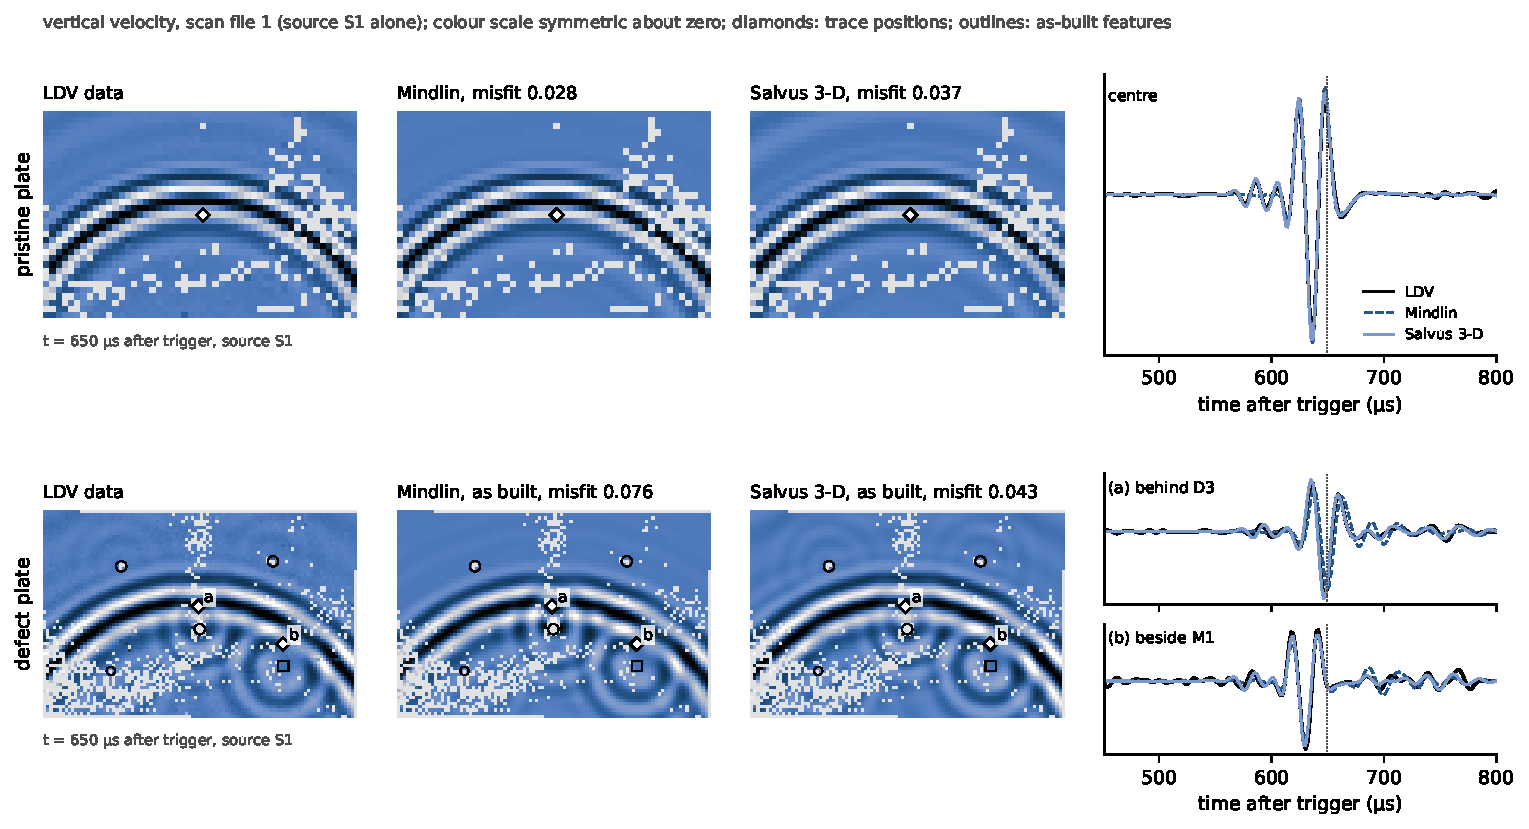
\includegraphics[width=\linewidth]{F3_waveforms.pdf}
\caption{\textbf{Forward-model check.} LDV vs Mindlin vs Salvus 3-D (full plate, free edges, PZT blocks, as-built holes and glued cube), same source-signature fit for every model; misfit over all files and points. Pristine plate: Mindlin 0.028 (calibrated on this scan), Salvus 0.037. Defect plate: Mindlin pristine 0.082, Mindlin as built (thinning, rigid cube) 0.076, Salvus as built 0.043, Mindlin blind inversion 0.042. The plate model is adequate for the intact plate; its representation of the through-hole and the glued mass is the weak point, which the blind inversion compensates with plugs.}\label{fig:forward}
\end{figure}

